\chapter{Basic Concepts}

\section*{What is Machine Learning?}

\begin{definitionblock}[Machine Learning]
\textbf{Machine Learning} is the science of getting computers to learn something without being explicitly programmed.
\end{definitionblock}

\begin{itemize}
    \item What science?
    \item Who is doing that?
    \item To learn what?
    \item Who is not being explicitly programmed?
\end{itemize}

Let's formalize the decision making process:

\begin{multicols}{2}
    \centering
    \texttt{$y = f(x)$}
    \columnbreak

    \begin{itemize}
        \item $x$ is the entity about which the decision has to be made
        \item $y$ is the decision
        \item $f$ is the procedure that, given an \curlyquotes{x} results in a decision \curlyquotes{y}
    \end{itemize}

\end{multicols}

X is an \textbf{observation}, while Y is a \textbf{response}.

So, the function $f$ is what has to be learned, and is also denoted as $f_{predict}$, since it predicts a response ($\hat{y}$) given an observation.

$$f: R^2 \to R$$

\begin{figure}[H]
    \centering
    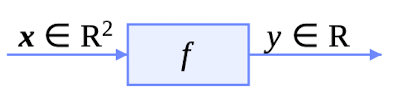
\includegraphics[width=0.3\textwidth]{assets/fig1.png}
    \caption{Abstract definition of the learning process}
    \label{fig:ML1}
\end{figure}

The learning process is not written by a human, so we can say that the machine learns \texttt{autonomously}.
\begin{itemize}
    \item condsider the universe of functions $F_{X \to Y} = \{f, f:X \to Y\}$
    \item choose the function that does what expected
\end{itemize}

\begin{definitionblock}[New Definition]
\textbf{Machine Learning} is the science of getting computers to learn $f_{predict}:X \to Y$ \textbf{autonomously}.
\end{definitionblock}

There has to be some sort of \texttt{supervision} facilitating the search of a good $f$ and when it is in the form of some \textbf{examples} and the function should process them correctly we are in the field of \textbf{Supervised Machine Learning}.
\begin{itemize}
    \item \textbf{Supervised Learning}: the function is learned from a set of labeled examples
    \item \textbf{Unsupervised Learning}: finds structures in the data without any labels
    \item \textbf{Reinforcement Learning}: the function is learned from a set of examples and a reward signal
\end{itemize}

Examples are pairs of observations and responses ($x,y$), and the set of examples is called \textbf{training set} (or learning set). The \texttt{dataset} is a bag of pairs of observations and responses.

The learning set has to be consistent with the domain and codomain of the function $f_{predict}$ to be learned.

$$f_{predict} = f_{learn}(D_{learn})$$

\begin{itemize}
    \item \textbf{learning phase}: the function $f_{learn}$ is learned from the learning set(i.e. is applied to obtain $f_{predict}$ from $D$)
    \item \textbf{prediction phase}: the function $f_{predict}$ is used to predict the response ($y$) of new observations
\end{itemize}

\begin{definitionblock}[Supervised Learning Technique]
A \textbf{Supervised Learning Technique} is a way to learn an $f_{predict} \in F_{X\to Y}$ given a $D_{learn} \in P^{*}(X \times Y)$
\end{definitionblock}

Different SL techniques differ in applicability, efficiency and effectiveness.
\begin{itemize}
    \item \textbf{Applicability}: with respect to X and\/or Y, e.g. some require $X = R^{p}$, some require $Y = R$
    \item \textbf{Efficiency}: the computational resources needed to learn the function wrt $|D_{learn}|$, e.g. some are fast and other slow
    \item \textbf{Effectiveness}: the quality of the learned functions $f_{predict}$
\end{itemize}

There is another view of it, and I like it more:
\begin{definitionblock}[SL Technique as Optimisation]
A \textbf{Supervised Learning Technique} is a way to solve the optimization problem:


$$f_{predict} = argmin_{f \in F_{X \to Y}} L(f, D_{learn})$$
    
where $L$ is a loss function that measures the quality of the function $f$ wrt the learning set $D_{learn}$ and $F_{X \to Y}$ is the set of functions that can be learned.
\end{definitionblock}

The most practical solution is to reduce $F_{X \to Y}$ size by considering only the $f$ of some nature.

\texttt{Templating $f$} means defining a relationship between data as we do in statistics, specifying it with some coefficients that we can evaluate.

We can then explicit the unknown parameters and specify the template as a reduced $F'$. 

$$f_{predict} = f'_{predict}(x,m)$$

Where $m$ is the \texttt{model} of how $y$ depends on $x$.

\begin{figure}[H]
    \centering
    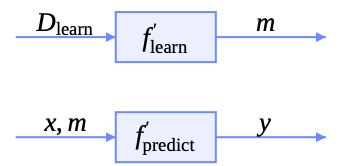
\includegraphics[width=0.3\textwidth]{assets/fig2.png}
    \caption{Learning a model with template function}
    \label{fig:template}
\end{figure}

\begin{definitionblock}[ML system]
An \textbf{information processing system} in which there is a SL technique and a pair of \textbf{pre-processing} and \textbf{post-processing} steps.
\end{definitionblock}

The designer of the ML system has to choose the learning technique, the pre/post processing steps and the relative parameters. The steps are:
\begin{itemize}
    \item Decide if to use a ML system
    \item Supervised vs Unsupervised vs Reinforcement
    \item Define the problem (X, Y, way of assessing solutions)
    \item Design the ML system (choose the ML technique, pre/post processing steps)
    \item Implement the ML system (learning/prediction phases, obtaining the data)
    \item Assess the system
\end{itemize}

